\documentclass[10pt, aspectratio=169]{beamer}
% Shared setup for every day of the course.
\usetheme[progressbar=frametitle, numbering=fraction, block=fill]{metropolis}
\usepackage[T1]{fontenc}
\usepackage[utf8]{inputenc}
\usepackage{lmodern}
\usepackage{amsmath, amssymb, bm, booktabs, graphicx, xcolor}
\usepackage{tikz}
\usetikzlibrary{arrows.meta, positioning, calc, shapes.geometric}

\graphicspath{{figures/}}

% --- colours -------------------------------------------------------------------------------------
\definecolor{accent}{HTML}{C0392B}
\definecolor{cool}{HTML}{2E6DB4}
\definecolor{muted}{HTML}{7A7A7A}
\definecolor{good}{HTML}{2E8B57}
\setbeamercolor{alerted text}{fg=accent}
\setbeamercolor{example text}{fg=cool}

% --- notation (follows the thesis' notation chapter) ---------------------------------------------
\newcommand{\given}{\,|\,}
\newcommand{\E}{\mathbb{E}}
\newcommand{\KL}[2]{D_{\mathrm{KL}}\!\left[#1\,\middle\|\,#2\right]}
\newcommand{\N}{\mathcal{N}}
\newcommand{\Hess}{\mathcal{H}}
\newcommand{\nats}{\,\text{nats}}
\DeclareMathOperator*{\argmin}{arg\,min}

% --- course devices ------------------------------------------------------------------------------
% \src{...}: where a claim or number comes from (thesis file and line, or a post-thesis note).
\newcommand{\src}[1]{\par\vfill\hfill{\scriptsize\color{muted}source: #1}}
% \wip: marks a post-thesis result.
\newcommand{\wip}{{\scriptsize\color{white}\colorbox{accent}{\,work in progress\,}}}
% \lesson{...}: the one sentence a frame exists to say.
\newcommand{\lesson}[1]{\begin{alertblock}{}\centering #1\end{alertblock}}
% a measurement story
\newenvironment{measured}[1]{\begin{exampleblock}{Measured: #1}}{\end{exampleblock}}

\author{Course built on the doctoral thesis of No\'e Zapata}
\institute{Montevideo, 30 November -- 4 December 2026}

% \cyclemap{n}: the course's five-stage cycle, stage n highlighted (1 room ... 5 memory).
\newcommand{\cyclemap}[1]{%
  \begin{tikzpicture}[
      st/.style={draw=muted, thick, rounded corners=3pt, fill=white, align=center,
                 minimum width=2.5cm, minimum height=0.8cm, font=\scriptsize, text=muted},
      on/.style={draw=accent, very thick, fill=accent!10, text=black, font=\scriptsize\bfseries},
      arr/.style={-{Stealth[length=2mm]}, thick, color=muted},
      s1/.style={}, s2/.style={}, s3/.style={}, s4/.style={}, s5/.style={}, s#1/.style={on}]
    \node[st, s1] (c1) at (90:1.9)   {estimate the room};
    \node[st, s2] (c2) at (18:2.6)   {localise; learn\\the body};
    \node[st, s3] (c3) at (-54:2.2)  {concepts fill\\the room};
    \node[st, s4] (c4) at (-126:2.2) {cross the door};
    \node[st, s5] (c5) at (162:2.6)  {new room;\\memory};
    \draw[arr] (c1) to[bend left=15] (c2); \draw[arr] (c2) to[bend left=15] (c3);
    \draw[arr] (c3) to[bend left=15] (c4); \draw[arr] (c4) to[bend left=15] (c5);
    \draw[arr] (c5) to[bend left=15] (c1);
  \end{tikzpicture}}


\title{A robot that acts to know}
\subtitle{Day 2 --- Estimating the room, and finding oneself in it}
\date{Tuesday 1 December}

\begin{document}

\maketitle

\begin{frame}{Where we are}
  \begin{columns}[c]
    \begin{column}{0.5\textwidth}
      \centering\cyclemap{1}
    \end{column}
    \begin{column}{0.48\textwidth}
      Yesterday the robot knew its pose, and we told it which points were the wall's.\\[0.6em]
      Today it knows neither:
      \begin{itemize}
        \item which points belong to which wall: \textbf{association};
        \item how many walls there are: \textbf{structure};
        \item where it is in the room it is building: \textbf{localisation}.
      \end{itemize}
      And every one of these is coupled to the others.
    \end{column}
  \end{columns}
\end{frame}

% =================================================================================================
\section{Two regimes}
% =================================================================================================

\begin{frame}{The room is either a variable or a constant}
  \begin{columns}[T]
    \begin{column}{0.48\textwidth}
      \begin{block}{Acquisition: the room is a variable}
        \small
        \begin{itemize}
          \item Walls $(\alpha_w,d_w)$ are unknowns, and so is their \emph{number}.
          \item Two poses that see one wall are coupled through it, so the graph has
                \textbf{cycles}.
          \item This is SLAM-like: poses and walls are solved together, and the solve
                \emph{terminates}.
        \end{itemize}
      \end{block}
    \end{column}
    \begin{column}{0.48\textwidth}
      \begin{block}{Operating: the room is a constant}
        \small
        \begin{itemize}
          \item The polygon is given; only the pose is estimated.
          \item The factors are unary, so the graph is a \textbf{chain}: the information matrix is
                banded and the solve is linear in the window length.
          \item The published covariance is over the pose alone.
        \end{itemize}
      \end{block}
    \end{column}
  \end{columns}
  \vspace{0.5em}
  \centering
  acquisition $\xrightarrow{\ \text{the polygon, exactly Manhattan}\ }$ operating
  \qquad
  operating $\xrightarrow{\ \text{the calibrated body}\ }$ acquisition
  \src{layout\_acquisition.tex l.131--174}
\end{frame}

\begin{frame}{Why split them? Because they change at different rates}
  \begin{itemize}
    \item A room changes when someone moves a wall: over years. A pose changes on every cycle.
    \item Estimating both jointly at frame rate, for ever, tracks a near-constant at great
          expense. It is the same category error as promoting a calibration constant to a state.
    \item So: \textbf{estimate jointly while the room is in question, then stop}, and hand over a
          \emph{settled} belief.
  \end{itemize}
  \pause
  \begin{alertblock}{The price}
    The operating regime cannot detect that the polygon it was given is wrong. The graph has no loop,
    so there is no loop closure: a systematic map error is absorbed into the poses while the
    reported covariance stays confident.
  \end{alertblock}
  You will measure this price in the lab.
  \src{layout\_acquisition.tex l.178--208}
\end{frame}

% =================================================================================================
\section{Acquiring the room}
% =================================================================================================

\begin{frame}{What is estimated}
  \footnotesize
  \begin{tabular}{@{}l p{0.42\textwidth} p{0.38\textwidth}@{}}
    \toprule
    quantity & what it is & why it is carried \\
    \midrule
    $\mathcal O$ & cyclic list of wall identifiers & it \emph{is} the topology; changing it
      changes the dimension of everything else \\
    $\alpha_w, d_w$ & each wall's line, $n(\alpha_w)^\top p = d_w$ & what the LiDAR constrains directly \\
    $\Lambda_w$ & each wall's $2\times2$ information & values the next look (Day 5) \\
    $[s_{\min},s_{\max}]_w$ & observed extent & a wall is a segment, not a line \\
    $e_w[i]$ & existence log-odds per 25 cm & a wall can be too \emph{long}, not just misplaced \\
    $k_w$, $\theta_0$ & Manhattan class, room direction & prefer right angles without forbidding others \\
    $X_t$ & five-pose window & walls are variables, so the poses must be solved with them \\
    \bottomrule
  \end{tabular}
  \vspace{0.6em}

  \normalsize The state is both \textbf{discrete} ($\mathcal O$, the number of walls) and
  \textbf{continuous} ($\alpha,d$). No number of Gauss--Newton steps changes a discrete
  variable, so a change of shape must be \emph{priced}.
  \src{layout\_acquisition.tex l.271--327}
\end{frame}

\begin{frame}{Whose frame? A gauge, and why it matters}
  \begin{itemize}
    \item With no map there is no world frame. The robot's frame at $t=0$ becomes the map frame.
    \item That is a \textbf{gauge}: a convention no measurement could ever fix, because the data
          would be identical in any other frame.
    \item The room's dominant direction $\theta_0$ is found by a \textbf{quadrupled-angle vote}:
          \[ \theta_0 = \tfrac14\arg\sum_i e^{4i\varphi_i}, \]
          which maps all four Manhattan normals onto one angle, so the vote needs no association.
  \end{itemize}
  \begin{measured}{a frame is part of an estimator's output \wip}
    A fitted room with area 23.88 m$^2$ against 24.00 true, but aspect ratio 1.344 against 1.500.
    The fit was fine; the \emph{frame} was wrong, because it was taken from the first scan. The
    cure: vote the gauge over all frames.
  \end{measured}
\end{frame}

\begin{frame}{Which points belong to a wall? A band that is derived, not chosen}
  \begin{columns}[c]
    \begin{column}{0.52\textwidth}
      \small
      Clutter is uniform over the area $A$. A wall concentrates its points in a strip $L$ long and
      about $\sigma$ wide:
      \[
        \frac{p_\text{wall}}{p_\text{clutter}} = \frac{A}{L\sqrt{2\pi}\,\sigma}\,e^{-r^2/2\sigma^2}
      \]
      \vspace{-0.6em}
      \begin{itemize}
        \item Inlier iff ratio $>1$: $r^2 < 2\sigma^2\ln\frac{A}{L\sqrt{2\pi}\sigma}$, about
              $3\sigma$.
        \item Each point brings $\ln(\text{ratio})$ \textbf{nats}.
        \item The band \textbf{narrows as $L$ grows}: a long wall is a more expensive explanation.
      \end{itemize}
    \end{column}
    \begin{column}{0.45\textwidth}
      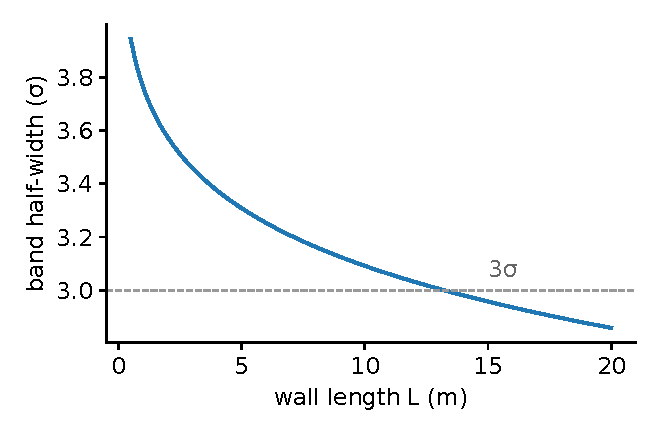
\includegraphics[width=\textwidth]{d2_band.pdf}
    \end{column}
  \end{columns}
  \lesson{A tuned threshold gives the band. The derivation gives the band \emph{and} the currency.}
  \src{layout\_acquisition.tex l.563--600}
\end{frame}

\begin{frame}{One scan, four walls}
  \begin{columns}[c]
    \begin{column}{0.45\textwidth}
      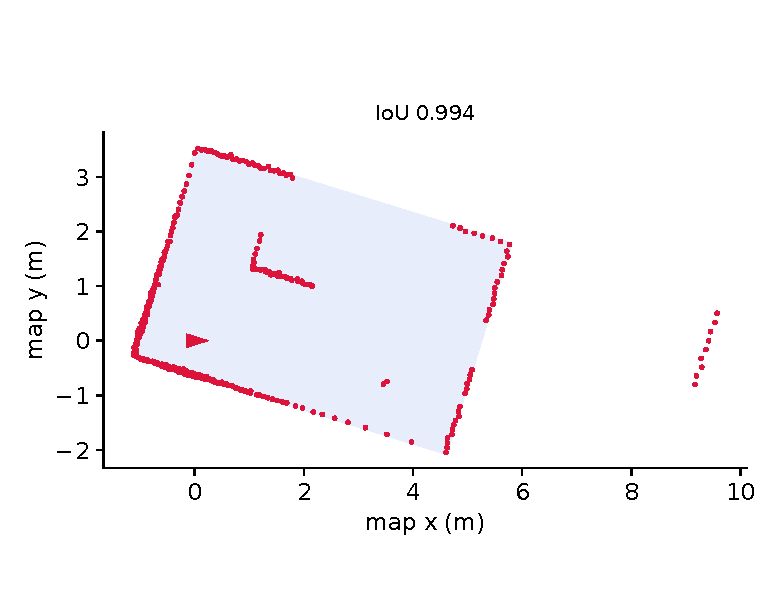
\includegraphics[width=\textwidth]{d2_room.pdf}
    \end{column}
    \begin{column}{0.52\textwidth}
      \small In the lab:
      \begin{enumerate}
        \item vote $\theta_0$ from local normals;
        \item initialise each class's $d$ from a median;
        \item refine each wall by a Laplace fit in which every point carries its
              \textbf{responsibility} $w=\rho/(1+\rho)$, entering with $\sigma/\sqrt{w}$;
        \item intersect the walls in cyclic order.
      \end{enumerate}
      The table, the bottle and the beams through the door are \emph{explained away as clutter}.
      Nobody wrote an \texttt{if}.
    \end{column}
  \end{columns}
\end{frame}

\begin{frame}{The price of a shape}
  A polygon with more sides always fits better. What stops the estimator adding them?\\[0.4em]
  \textbf{Minimum description length.} To transmit one edge, say its Manhattan direction and its
  offset at the sensor's resolution:
  \[
    L_\text{edge} = \ln 4 + \ln\frac{2R}{c} = 1.386 + 5.298 = 7.29\nats
    \qquad (R=10\text{ m},\ c=8\text{ cm}).
  \]
  \begin{itemize}
    \item An oblique edge names its angle instead of its class: a surcharge of $5.7$ nats. Manhattan
          is \emph{preferred}, not imposed.
    \item The old design had a hand-tuned 15 nats for a two-edge change. The derivation gives
          $14.6$. It does not refine the constant; it \alert{explains} it.
    \item The price depends on the instrument ($R$, $c$), not on the room. That is where it
          belongs.
  \end{itemize}
  \src{layout\_acquisition.tex l.702--738}
\end{frame}

\begin{frame}{But the table pays the price, too}
  \begin{itemize}
    \item In the lab, the table's south face earns about \textbf{80 nats} as a candidate wall,
          against a price of 7.6. Face evidence alone would make the table part of the room.
    \item What tells a table face from a wall is \textbf{free space}: beams pass beside and beyond
          it and hit the real wall behind it.
    \item Hence two evidence channels, kept apart: face evidence, and a free/occupied grid. A
          single-number grid once marked 38 of 42 cells of a 13 cm wall as free.
  \end{itemize}
  \begin{measured}{the layout is a box cover of free space \wip}
    Constructing the room from swept free space beat fitting a hull and repairing it on 8 of 9
    test rooms (worst case 0.872 $\to$ 0.940 IoU). Free space must be charged both ways: area
    claimed but never swept, \emph{and} area swept but not claimed.
  \end{measured}
  \src{layout\_acquisition.tex l.329--415}
\end{frame}

% =================================================================================================
\section{Localisation is one more belief}
% =================================================================================================

\begin{frame}{The observation model: no rendering}
  For a scan $\{p_i\}$ in robot coordinates and a candidate pose $X=(R(\phi),t)$:
  \[
    d_i(X) = \operatorname{dist}\big(R(\phi)p_i + t,\ \text{polygon}\big),
    \qquad
    \mathcal L_\text{obs} = \frac{1}{2\sigma^2}\cdot\frac1N\sum_i w_i\,\mathrm{Huber}(d_i)
  \]
  \begin{itemize}
    \item The residual \emph{is} the prediction error: no expected scan is rendered. Its Jacobian is
          the gradient of the distance field.
    \item $w_i^\text{range}\propto r_i^\alpha$: far returns have more leverage on heading.
          $w_i^\text{inc}=|\hat r_i\cdot\hat n_i|^\beta$: Day 1's incidence lesson.
    \item Note the $\frac1N$. The term is a \textbf{mean}, so its precision does not grow with
          scan density. Keep that in mind until the end of the day.
  \end{itemize}
  \src{room\_concept.tex l.241--310}
\end{frame}

\begin{frame}{What the residual floor is made of}
  Park the robot. The mean wall distance of each new scan hovers near \textbf{87 mm}, and never
  reaches zero.
  \begin{itemize}
    \item The fluctuation is white, and follows $N^{-1/2}$: measured ratio $1.41$ against a
          predicted $\sqrt{405/200}=1.42$.
    \item Solved backwards, that gives a per-point scatter of $\approx 37$ mm, which accounts for
          $0.798\times 37\approx 30$ mm of the floor.
    \item The other $\approx 57$ mm is \textbf{map mismatch}: the room is not exactly the polygon.
  \end{itemize}
  \lesson{Two-thirds of the floor is an error every return shares. More returns cannot remove it.}
  \src{room\_concept.tex l.385--425}
\end{frame}

\begin{frame}{Predict honestly: no constant process noise}
  Between scans the pose is propagated by odometry:
  \[
    \Sigma_{t+1} = F\,\Sigma_t F^\top + G\,\mathrm{diag}(\sigma_v^2,\sigma_\omega^2)\,G^\top
  \]
  \begin{itemize}
    \item $F,G$: Jacobians of the motion with respect to the pose and to the measured $(v,\omega)$.
    \item The covariance grows because of what the encoders and gyro cannot tell, \emph{not} by
          adding a constant $Q$ every cycle.
    \item In the lab, dead reckoning with this model is calibrated: normalised errors have
          standard deviations of $1.13, 0.99, 1.07$, against 1 if honest.
  \end{itemize}
  A constant $Q$ is a modelling decision dressed as a tuning knob. On Day 4 we will meet the
  pathology it causes in object beliefs.
\end{frame}

\begin{frame}{Localising against the room you just built}
  \begin{columns}[c]
    \begin{column}{0.5\textwidth}
      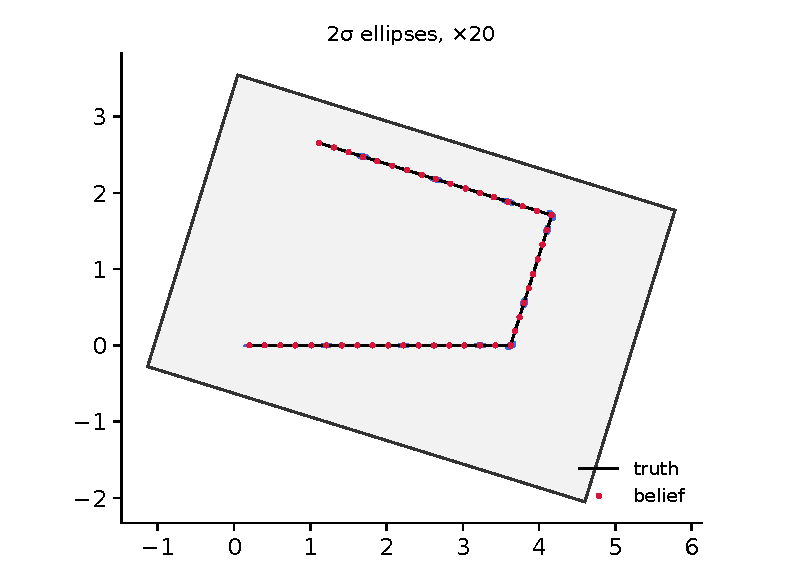
\includegraphics[width=\textwidth]{d2_track.pdf}
    \end{column}
    \begin{column}{0.48\textwidth}
      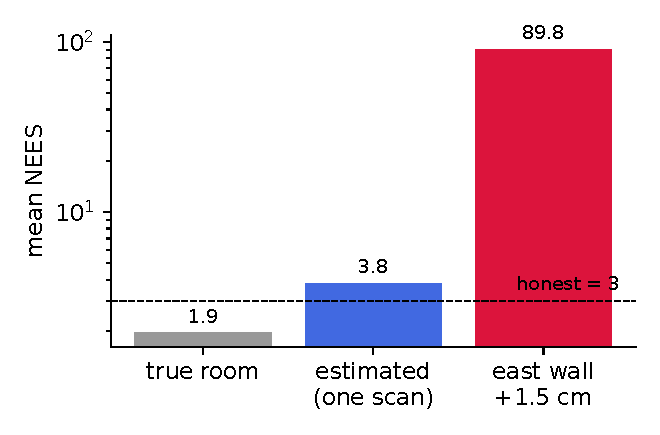
\includegraphics[width=\textwidth]{d2_nees.pdf}
      \small
      A wall \textbf{1.5 cm} out of place makes the localiser confidently wrong: NEES 90 where 3 is
      honest.
    \end{column}
  \end{columns}
  \lesson{In the operating regime the polygon is a constant, so its error is shared by every scan,
          for ever.}
\end{frame}

\begin{frame}{Symmetry: where descent cannot help}
  \begin{columns}[c]
    \begin{column}{0.45\textwidth}
      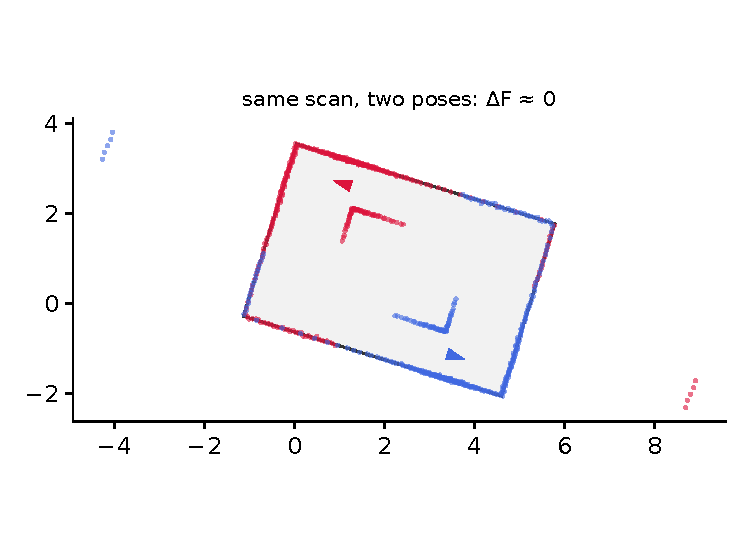
\includegraphics[width=\textwidth]{d2_symmetry.pdf}
    \end{column}
    \begin{column}{0.53\textwidth}
      \small
      \begin{itemize}
        \item A rectangle looks the same after a half-turn. The same scan fits both poses with
              \emph{identical} free energy.
        \item No downhill path joins them. They are \textbf{separate hypotheses}, so the agent
              must enumerate them and choose: a coarse search over the room's symmetries, then local
              refinement.
        \item This is one of the few places where a threshold is right: \emph{a threshold is
              defensible exactly when the alternative cannot be expressed as a covariance.}
        \item What breaks the tie must be evidence the room does not contain: the motion prior, or
              an asymmetric landmark (the thesis uses the fridge).
      \end{itemize}
    \end{column}
  \end{columns}
  \src{room\_concept.tex l.1867--1927}
\end{frame}

% =================================================================================================
\section{Shared error}
% =================================================================================================

\begin{frame}{The common-mode ceiling}
  $N$ residuals $r = r_0 + J_z\delta + \varepsilon$ that share one offset $\delta\sim\N(0,\Sigma_\delta)$
  (a pose error), plus independent noise $\varepsilon\sim\N(0,\sigma^2 I)$. Marginalise $\delta$:
  \[
    \mathcal I = J_z^\top\big(\sigma^2 I + J_z\Sigma_\delta J_z^\top\big)^{-1}J_z
    \;\overset{\text{Woodbury}}{=}\;
    \big(\sigma^2(J_z^\top J_z)^{-1} + \Sigma_\delta\big)^{-1}
    \;\xrightarrow[N\to\infty]{}\; \Sigma_\delta^{-1}
  \]
  \begin{itemize}
    \item A denser mask eventually stops helping. The ceiling is set by the \emph{pose} error, not
          by the pixel count.
    \item The joint information on (object, offset) has rank 6, not 12: the data cannot tell a
          displaced object from a displaced robot. Only the ceiling is computable.
  \end{itemize}
  \src{concept\_agents.tex l.1047--1090}
\end{frame}

\begin{frame}{The ceiling, measured in the toy}
  \begin{columns}[c]
    \begin{column}{0.48\textwidth}
      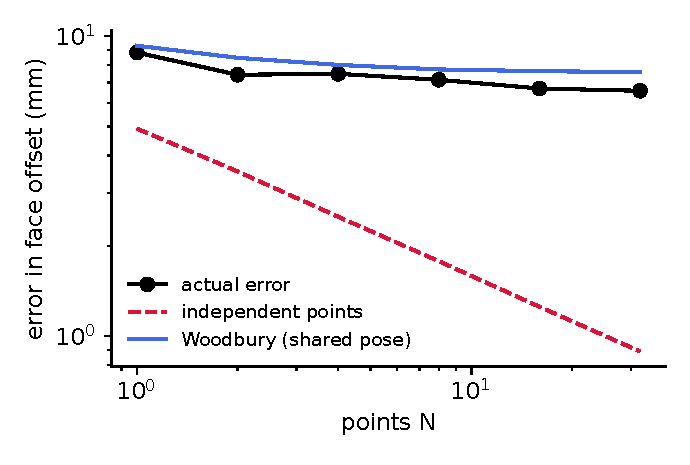
\includegraphics[width=\textwidth]{d2_ceiling.pdf}
    \end{column}
    \begin{column}{0.5\textwidth}
      \small
      The robot maps the table's face from a \emph{dead-reckoned} pose, before it has a room to
      localise against: exactly the situation while a room is still being estimated.
      \begin{itemize}
        \item Treating points as independent claims under 1 mm at $N=32$.
        \item The real error stalls near 7 mm.
        \item Woodbury predicts it to within about 10\% at every $N$.
      \end{itemize}
    \end{column}
  \end{columns}
  \lesson{Averaging removes independent error. It does not remove shared error.}
\end{frame}

\begin{frame}{Case study: association dies by a common-mode latch \wip}
  \begin{columns}[T]
    \begin{column}{0.5\textwidth}
      \small One frame of a real recording, four walls still associating:\\[0.3em]
      \footnotesize
      \begin{tabular}{@{}c r r r@{}}
        \toprule
        seg & $\chi^2$ & $\Delta\phi$ & gate $\sigma_\phi$ \\
        \midrule
        0 & 1.03 & $-5.85^\circ$ & $6.78^\circ$ \\
        1 & 1.02 & $-5.76^\circ$ & $6.34^\circ$ \\
        2 & 1.20 & $-5.79^\circ$ & $6.01^\circ$ \\
        3 & 1.06 & $-5.77^\circ$ & $6.67^\circ$ \\
        \bottomrule
      \end{tabular}
    \end{column}
    \begin{column}{0.48\textwidth}
      \small
      \begin{itemize}
        \item The \emph{same} $-5.8^\circ$ on every wall is one \textbf{heading} error, not four
              wall errors.
        \item Each wall is gated independently against an error they all share. When the common
              error crosses $\approx 6^\circ$, they all fail \alert{in the same frame}.
        \item With nothing associated, nothing is left to correct the pose: 100\% $\to$ 0\%,
              permanently.
      \end{itemize}
    \end{column}
  \end{columns}
  \vspace{0.4em}
  \small Parked runs never accumulate 6°, which is why ``a parked run looks perfect and the first
  tour kills it''.
  \src{post-thesis note, 2026-09-18}
\end{frame}

\begin{frame}{Case study: the pose must not lean on a room still being built \wip}
  While the room was being estimated, the pose was registered against the \emph{provisional}
  layout. Layout errors dragged the pose; the dragged pose corrupted the layout.
  \vspace{0.3em}
  \begin{center}\small
  \begin{tabular}{@{}l r r r@{}}
    \toprule
    pose error (median, vs ground truth) & run A & run B (20 min) & run C (wheel slip) \\
    \midrule
    registered to the provisional layout & 0.22 m & 3.13 m & 1.55 m \\
    odometry alone                        & 0.08 m & 0.20 m & 1.77 m \\
    plain scan-to-map SLAM                & 0.010 m & 0.013 m & 0.031 m \\
    \bottomrule
  \end{tabular}
  \end{center}
  \begin{itemize}\small
    \item The fix: take the pose from plain SLAM, and build the layout \emph{from} the aligned map.
    \item Live in simulation: pose median 6 mm; layout IoU 0.896 at 20 s and 0.956 at 60 s.
    \item Registering to the provisional layout was \emph{worse than odometry alone}: a factor
          inherits the errors of whatever it is estimated through (Day 1).
  \end{itemize}
  \src{post-thesis note, 2026-10-09}
\end{frame}

% =================================================================================================
\section{Lab}
% =================================================================================================

\begin{frame}{Lab 2: the room, the pose, and the ceiling}
  \texttt{labs/day2.ipynb}, about 75 minutes. No labels, no known pose.
  \begin{enumerate}\small
    \item[A.] \textbf{Acquire}: the 4$\theta$ vote; the derived band; four walls by
              responsibility-weighted Laplace fits; the polygon and its IoU. MDL: does the table pay
              the price?
    \item[B.] \textbf{Localise}: the pose residual; drive the route; NEES against the true room, the
              estimated room, and a room with one wall 1.5 cm out.
    \item[C.] \textbf{Symmetry}: $F$ at the true pose and at its half-turn. What breaks the tie?
    \item[D.] \textbf{Ceiling}: map the table face from a dead-reckoned pose; actual error vs
              independent vs Woodbury.
  \end{enumerate}
\end{frame}

\begin{frame}{Tomorrow}
  \begin{columns}[c]
    \begin{column}{0.55\textwidth}
      Today the robot's odometry was honest. Tomorrow it is not: its wheels over-report by a few
      per cent and its gyro drifts. Nobody tells it so.\\[0.5em]
      It will discover its own body from the corrections the room supplies, learn which motions
      reveal which parameters, and find that standing still is sometimes the most informative
      thing it can do.
    \end{column}
    \begin{column}{0.42\textwidth}
      \begin{block}{Reading for Day 3}\small
        Thesis chapter \emph{Self-Calibration of the Robot's Body}: ``What the body is'', ``What no
        data can determine'', ``What each motion makes observable''.
      \end{block}
    \end{column}
  \end{columns}
\end{frame}

\end{document}
